\documentclass[aspectratio=169]{beamer}

\usepackage[utf8]{inputenc}


%Information to be included in the title page:
\title{Modeling Urban-Rural Poverty}
\author{Matthew Cooper}
\institute{World Data Lab}
\date{January 2021}



\begin{document}

\frame{\titlepage}

\begin{frame}
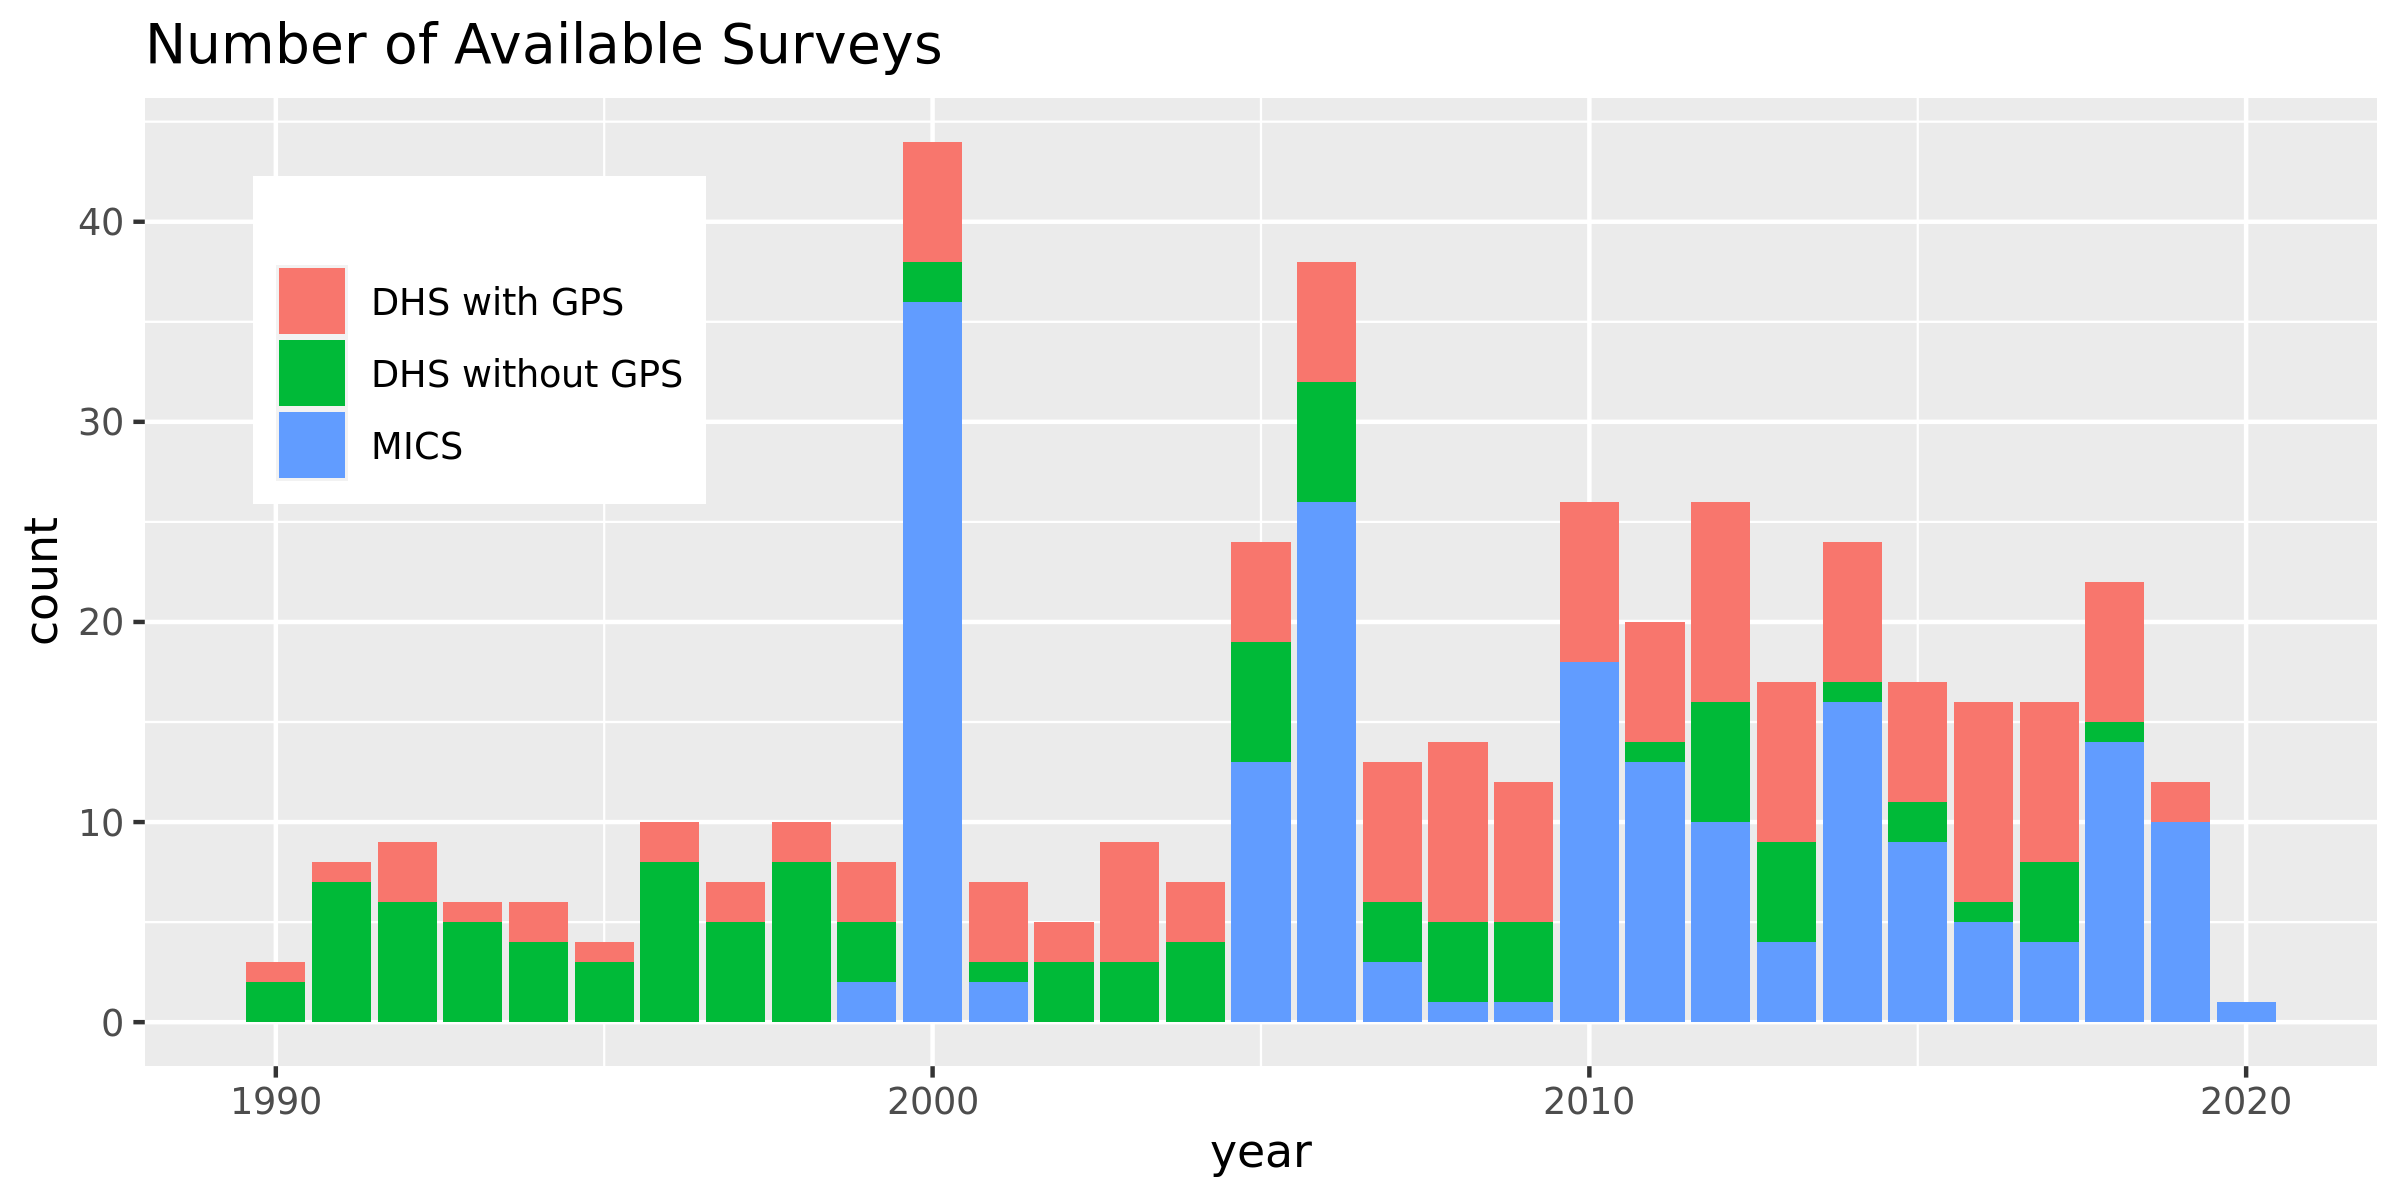
\includegraphics[width=\textwidth]{../res/Survey_count_time.png}
\end{frame}

\begin{frame}
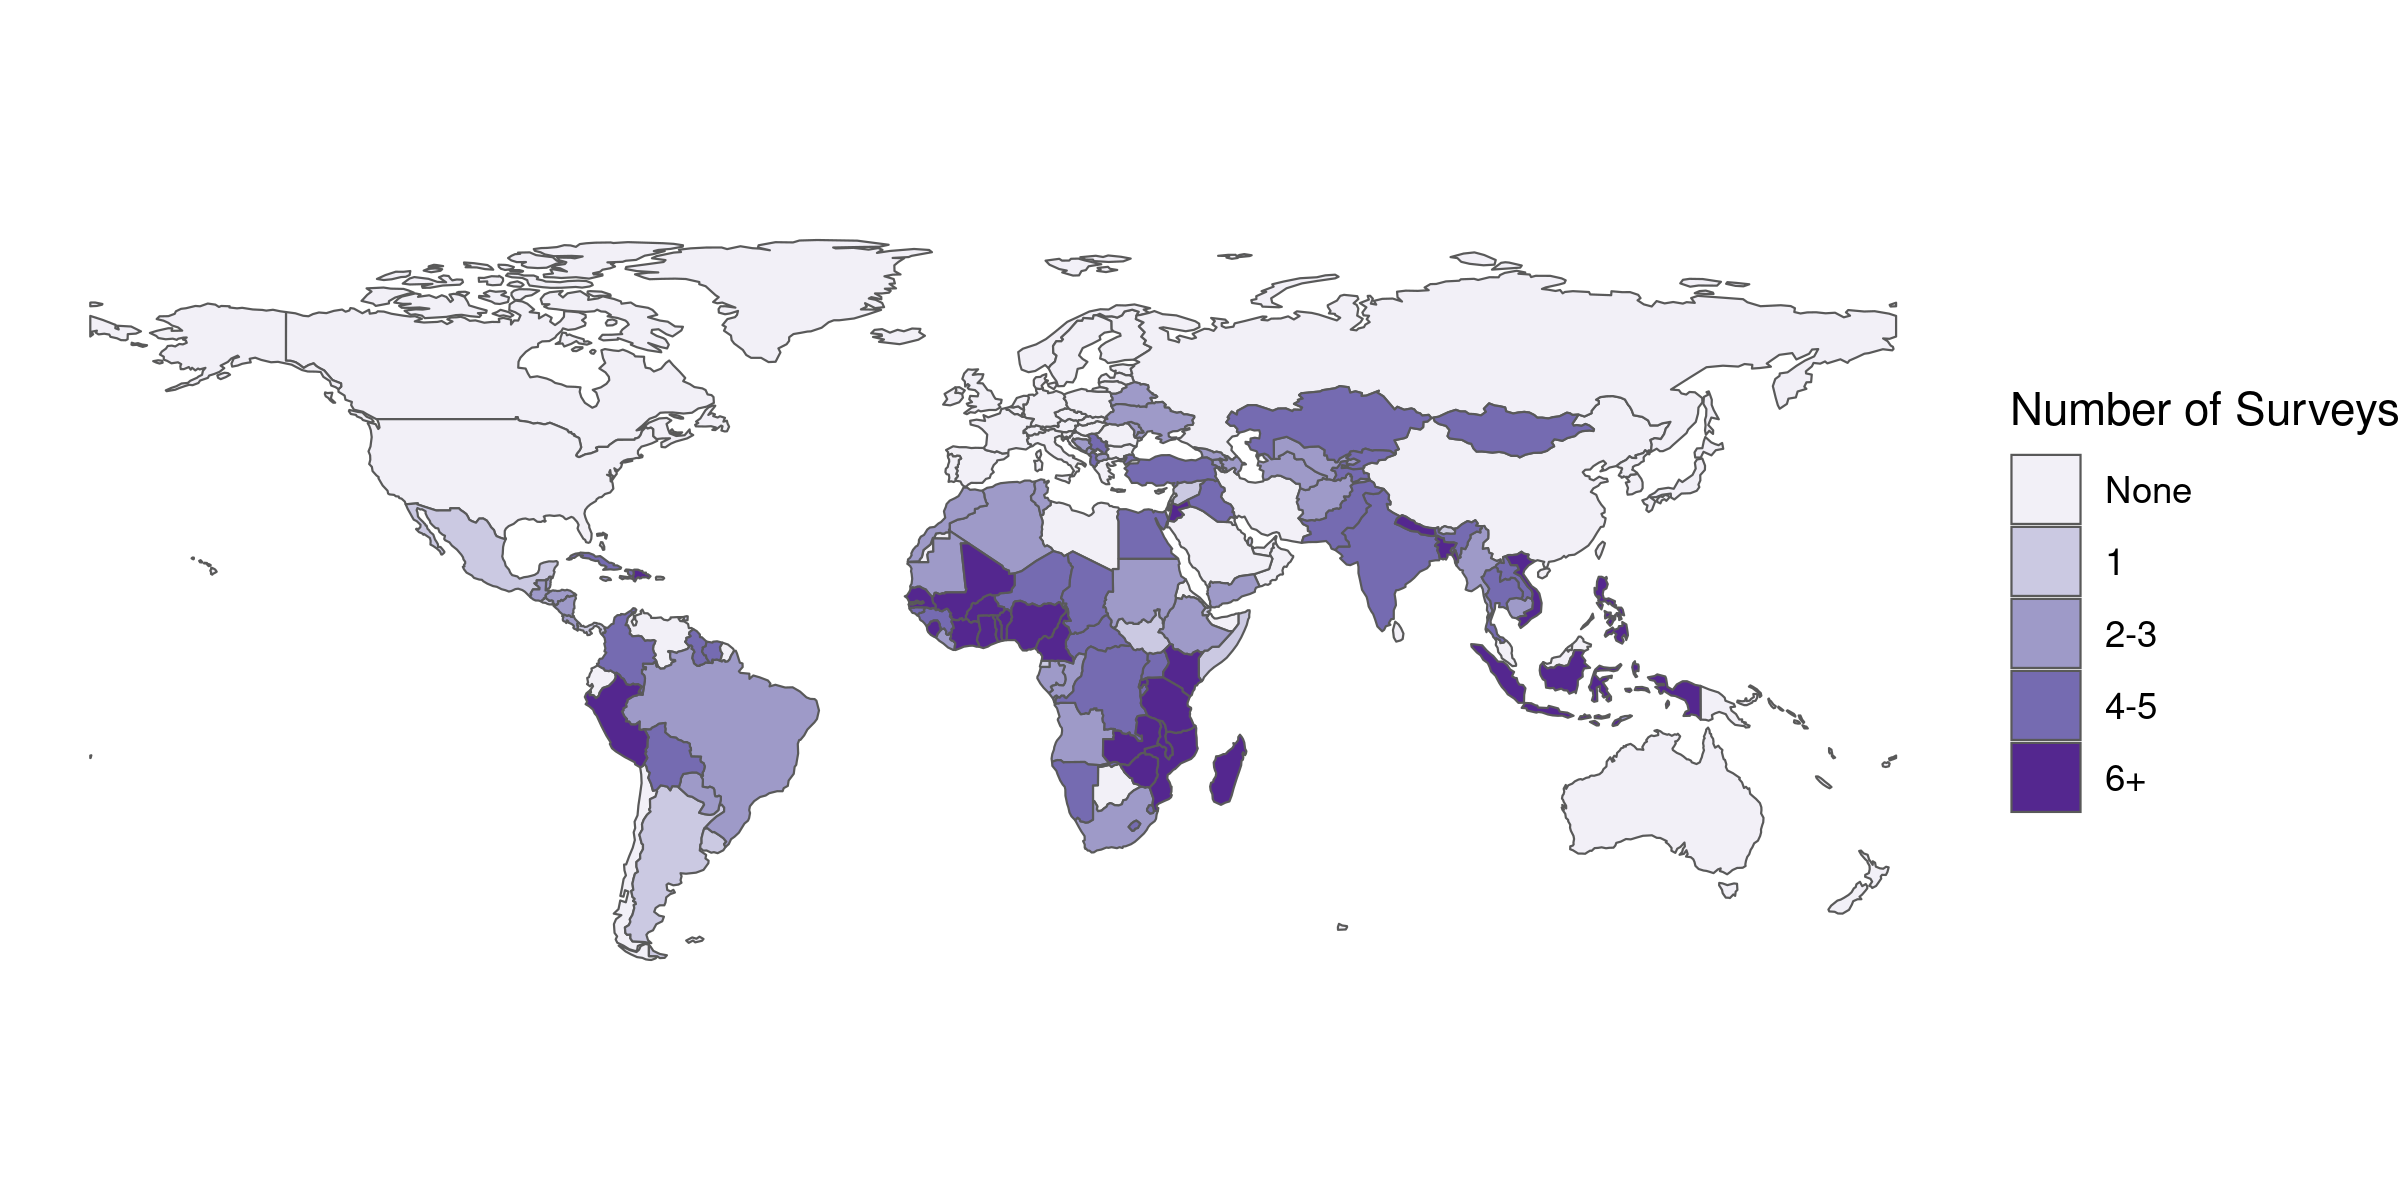
\includegraphics[width=\textwidth]{../res/Survey_count_space.png}
\end{frame}

\begin{frame}

Run principle component analysis on the following items:

\begin{enumerate}
	\item Sanitation
    \begin{enumerate}
        \item toilet type
        \item drinking water source
    \end{enumerate}
  \item Housing
    \begin{enumerate}
        \item wall materials
        \item floor materials
        \item roof materials
        \item number of sleeping rooms
    \end{enumerate}
  \item Possessions
    \begin{enumerate}
        \item has electricity
        \item has radio
        \item has television
        \item has refrigerator
        \item has bicycle
        \item has motorcycle
        \item has car
        \item toilet type
        \item drinking water source
    \end{enumerate}
\end{enumerate}
\end{frame}

\begin{frame}
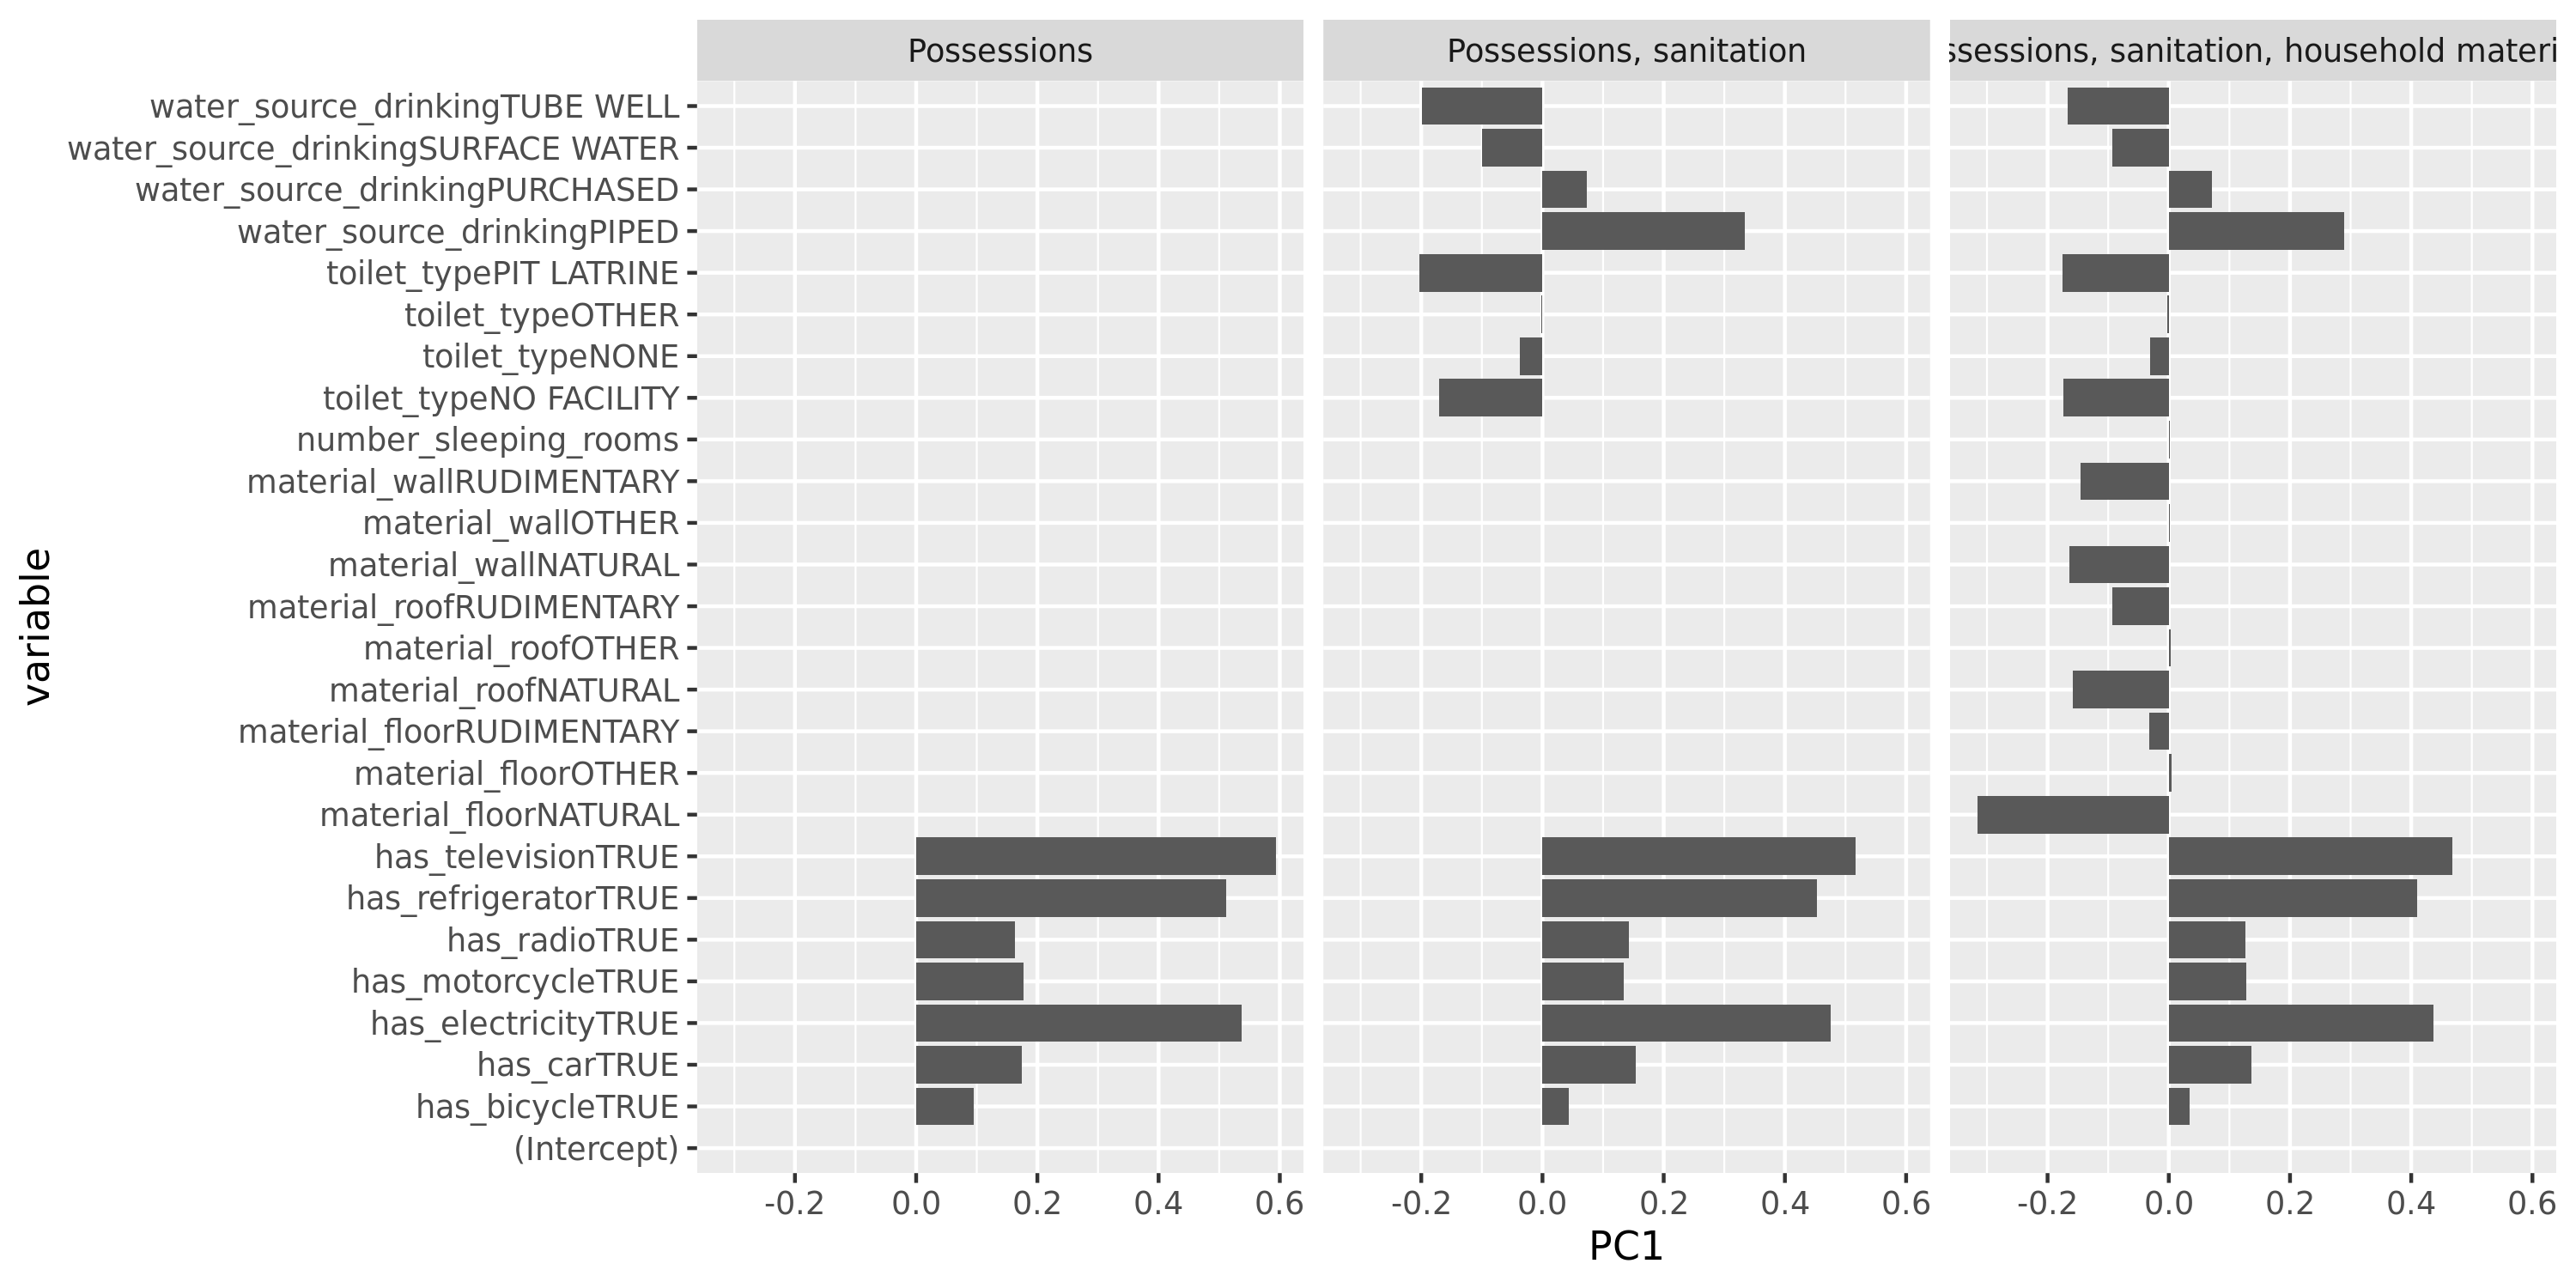
\includegraphics[width=\textwidth]{../res/PCA_loadings.png}
\end{frame}

\begin{frame}
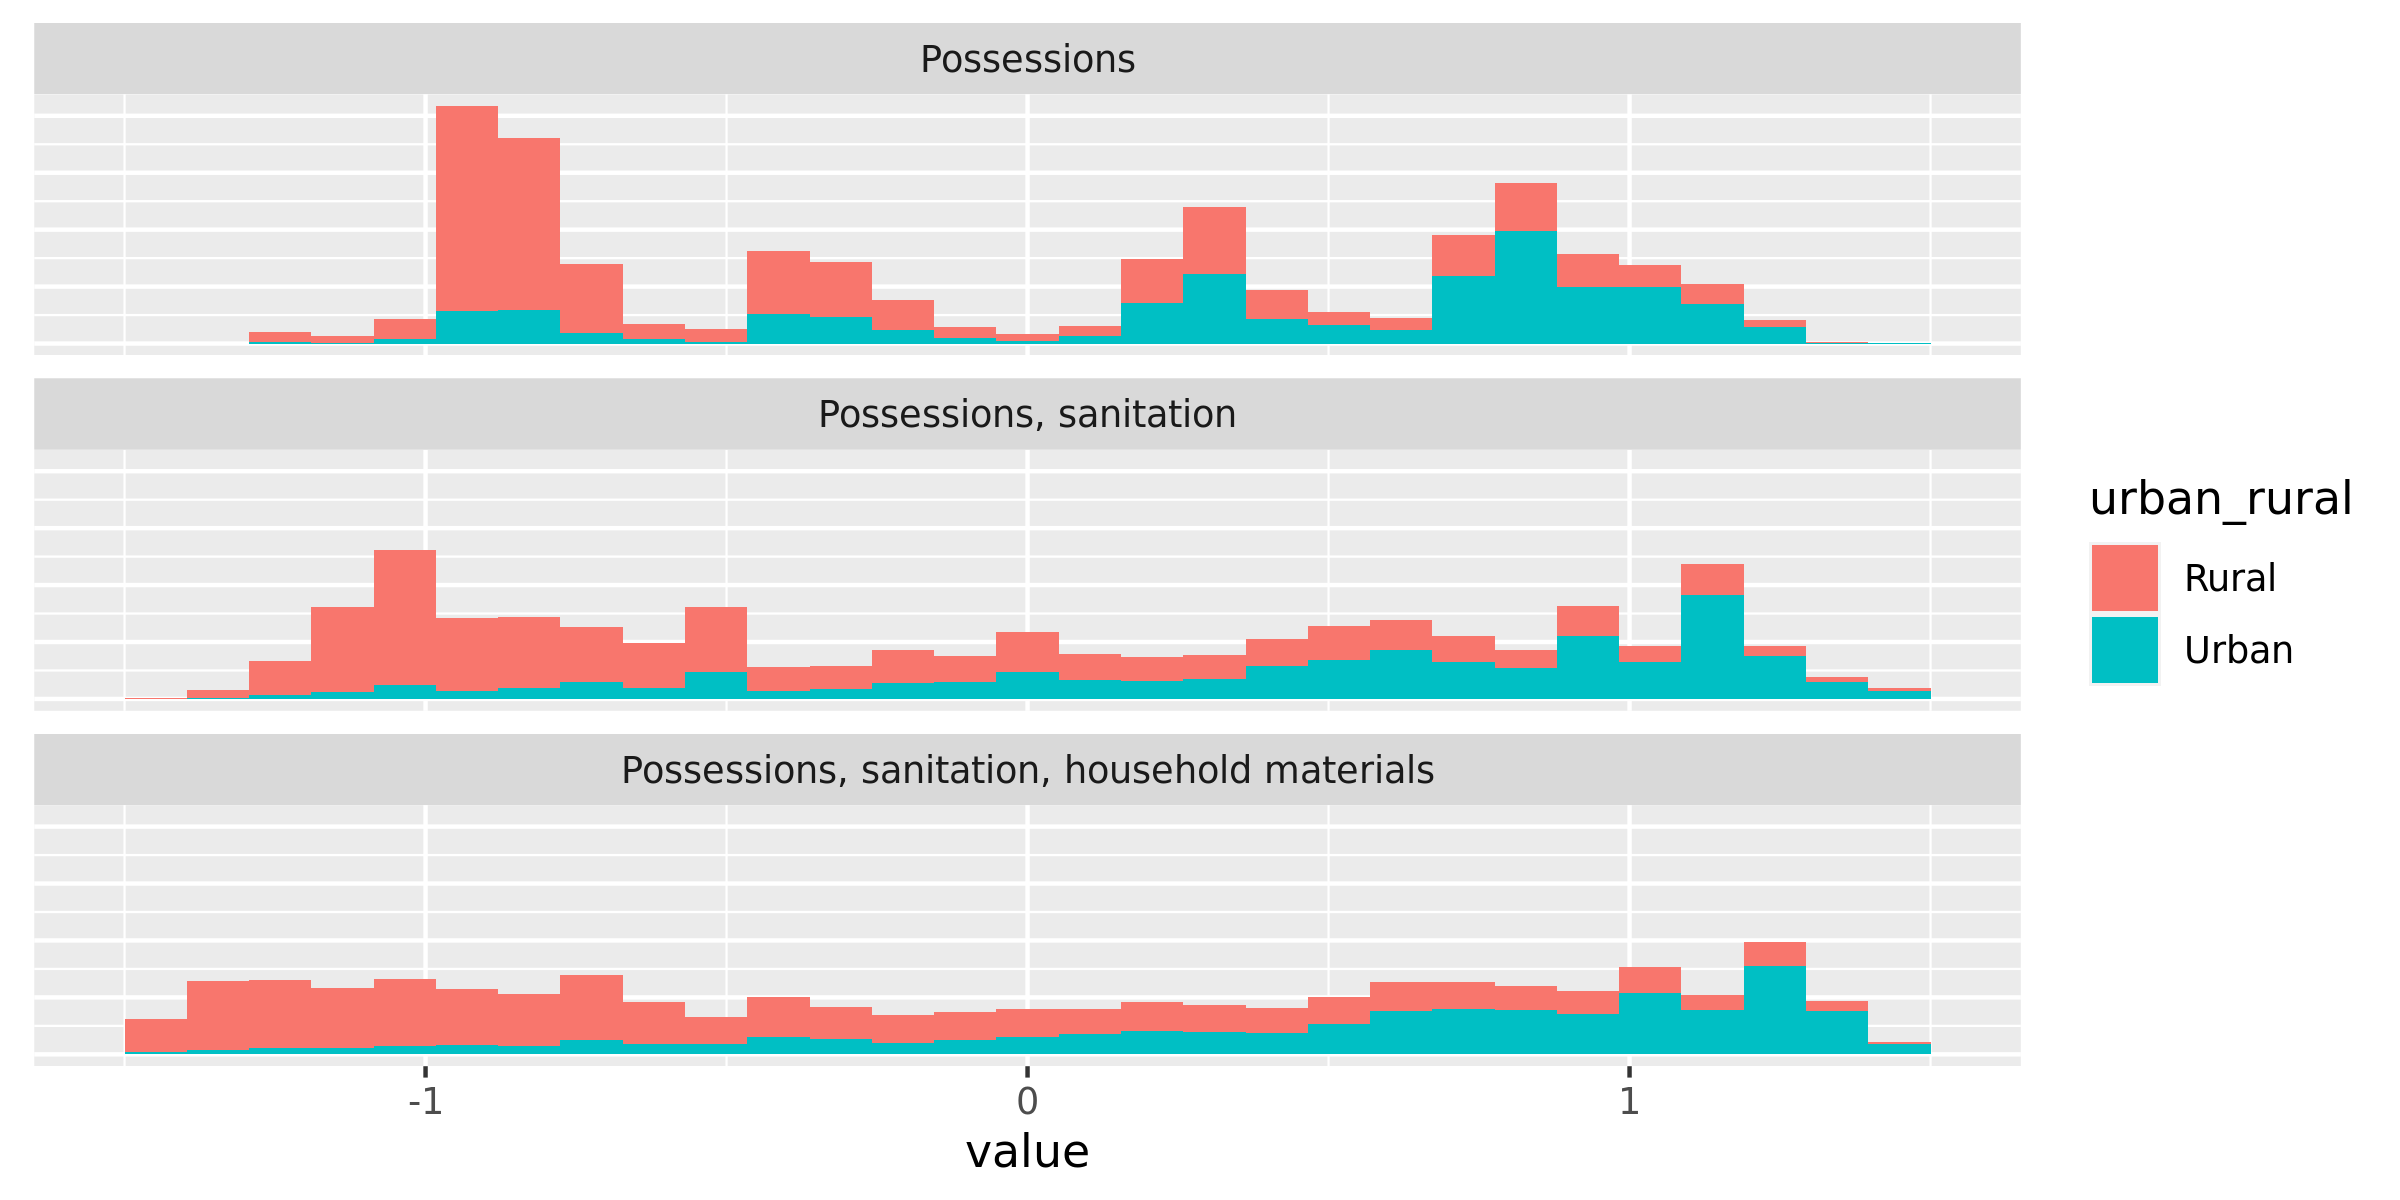
\includegraphics[width=\textwidth]{../res/urban_rural_histograms.png}
\end{frame}

\begin{frame}
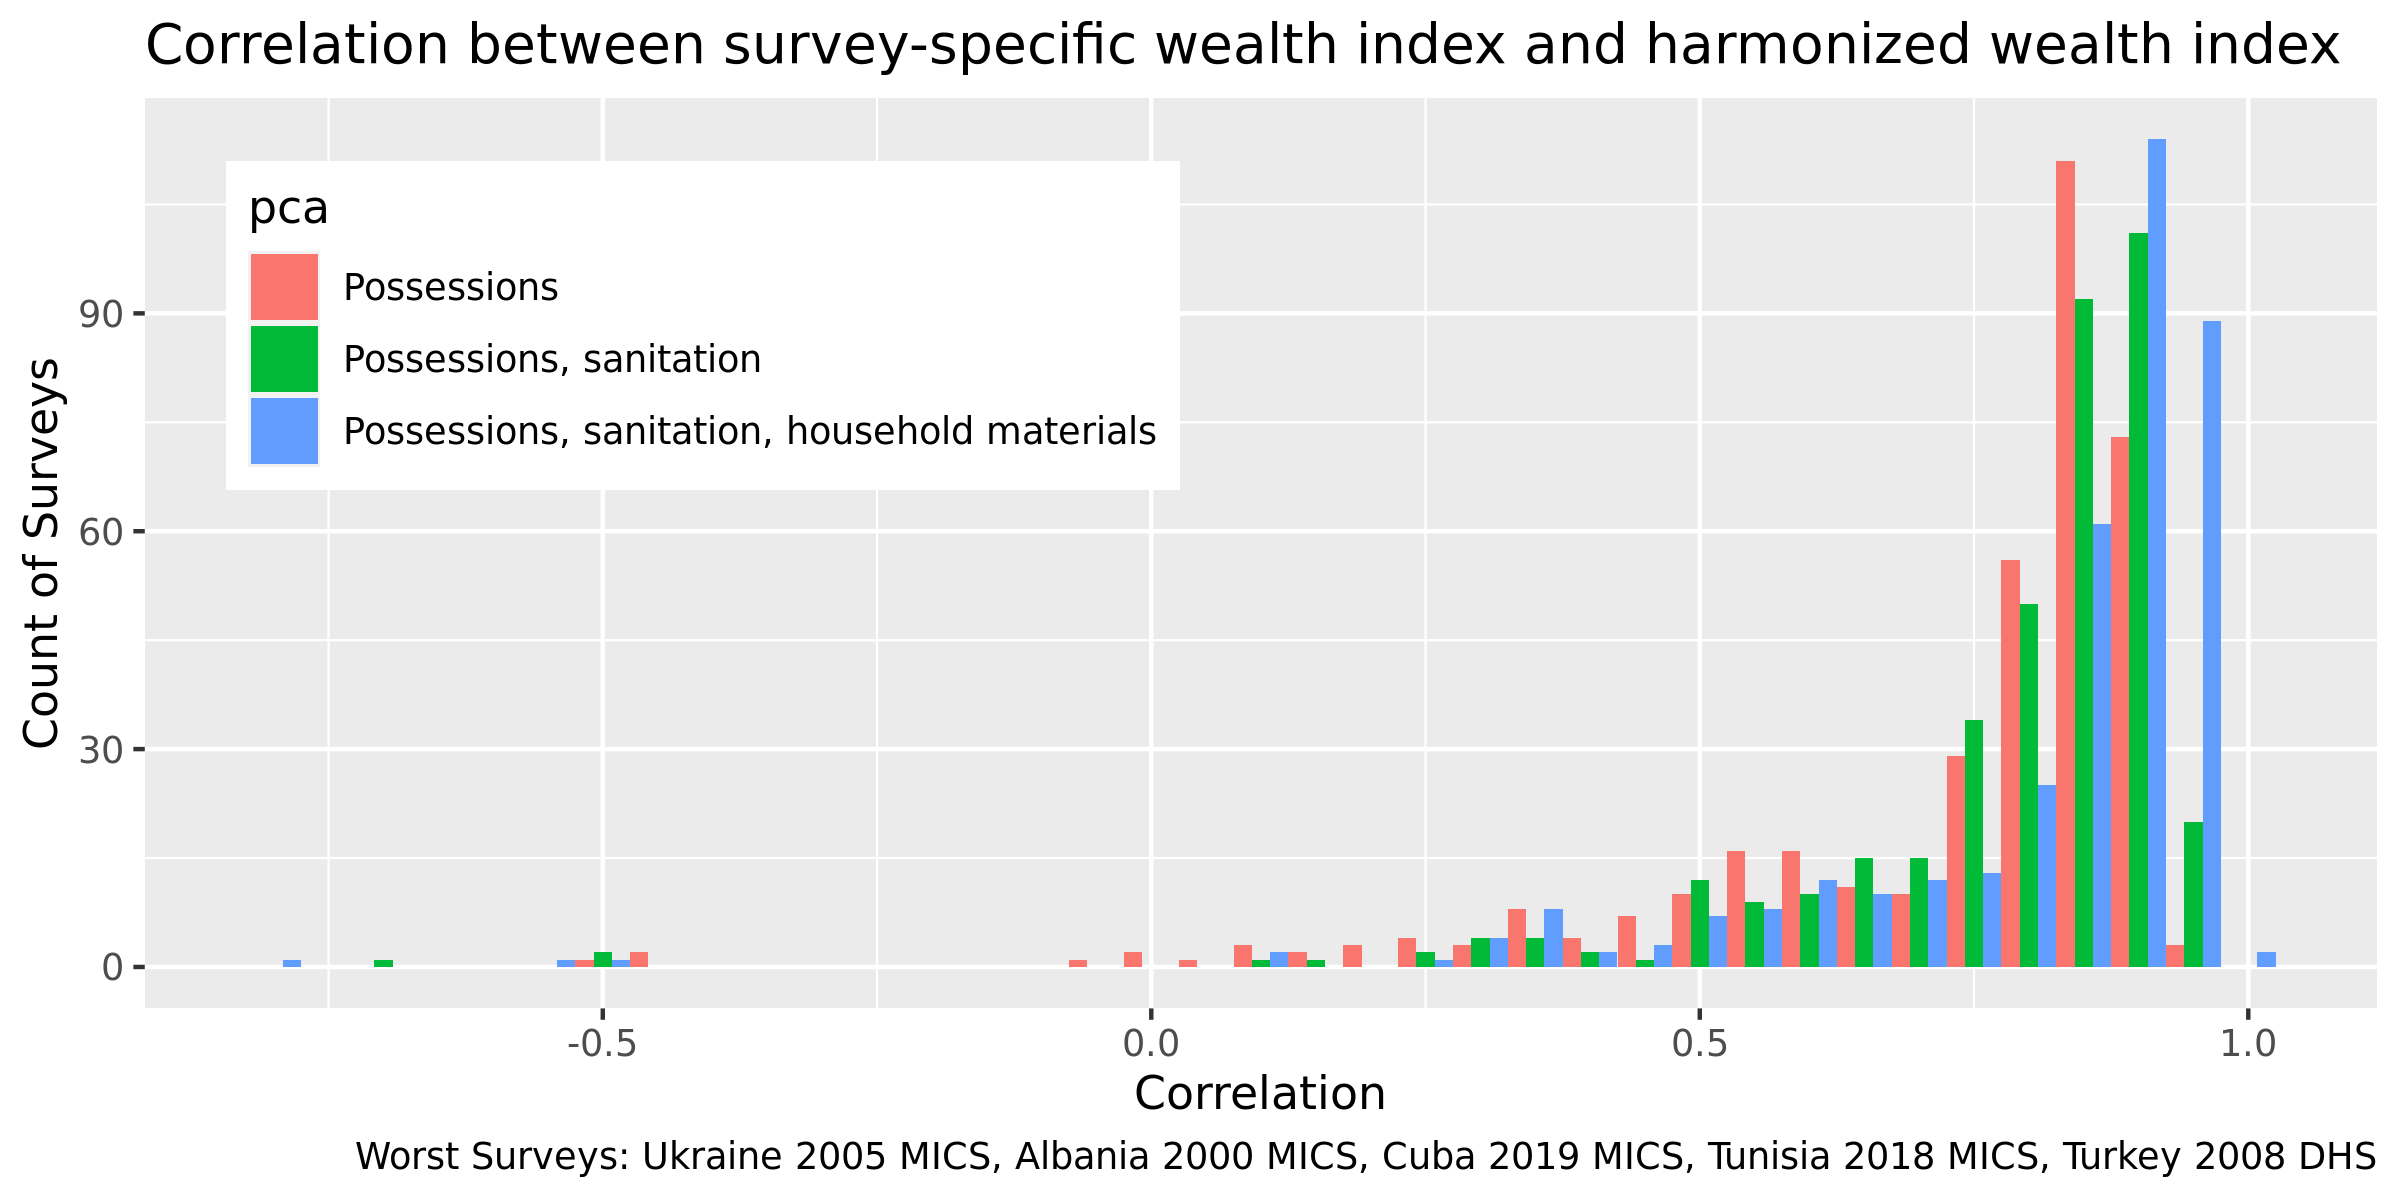
\includegraphics[width=\textwidth]{../res/correlation_histogram_all.png}
\end{frame}

\begin{frame}
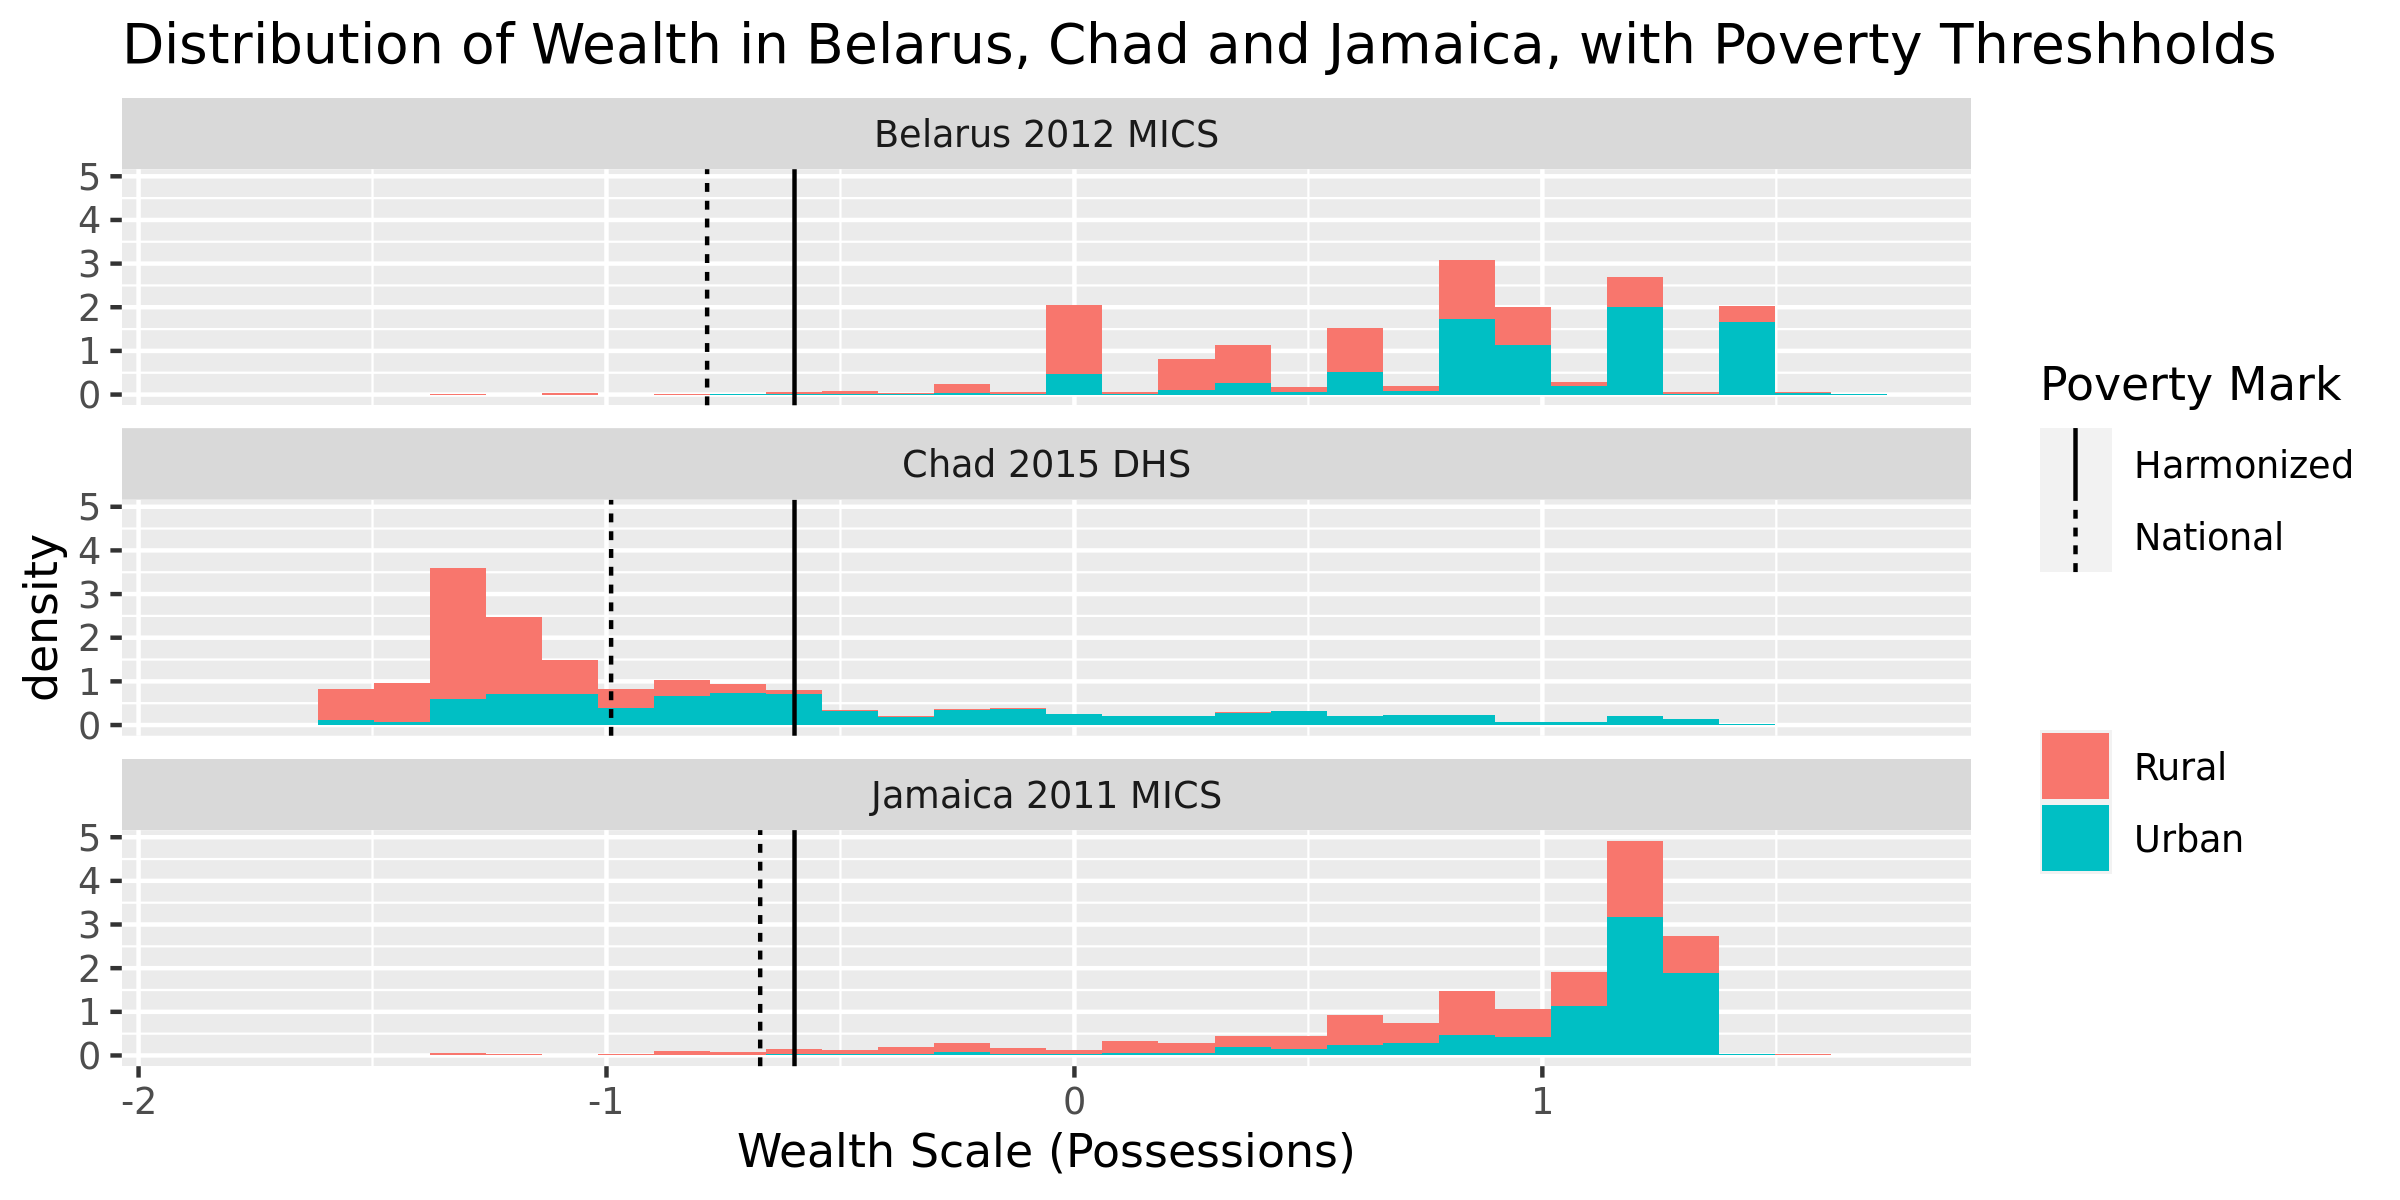
\includegraphics[width=\textwidth]{../res/example_histogram_multiple.png}
\end{frame}

\begin{frame}
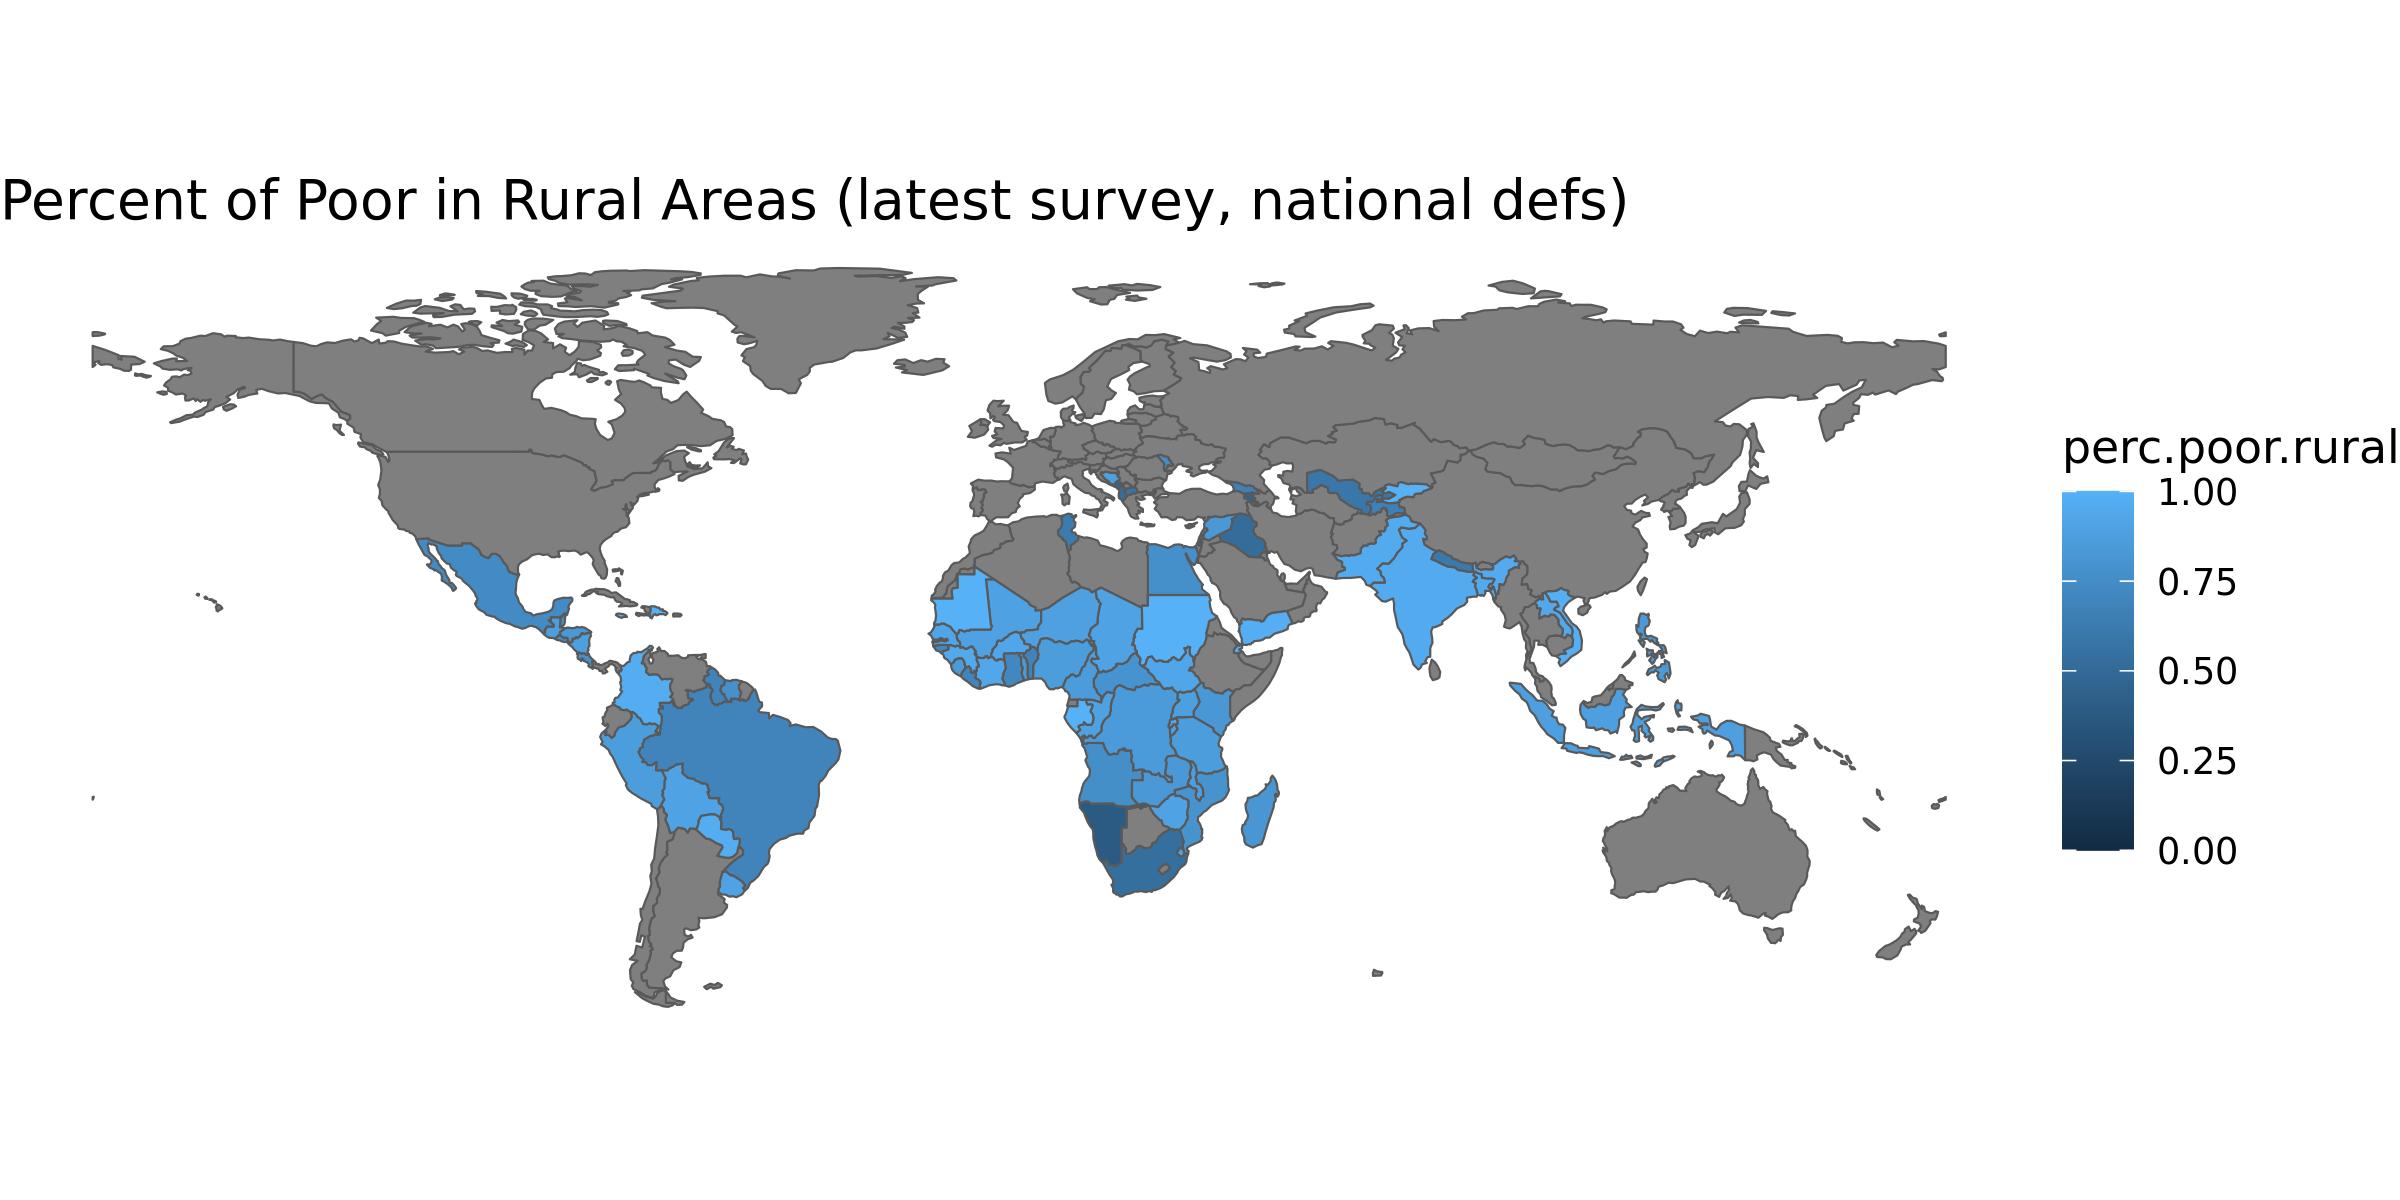
\includegraphics[width=\textwidth]{../res/perc.poor.rural_nat.png}
\end{frame}

\begin{frame}
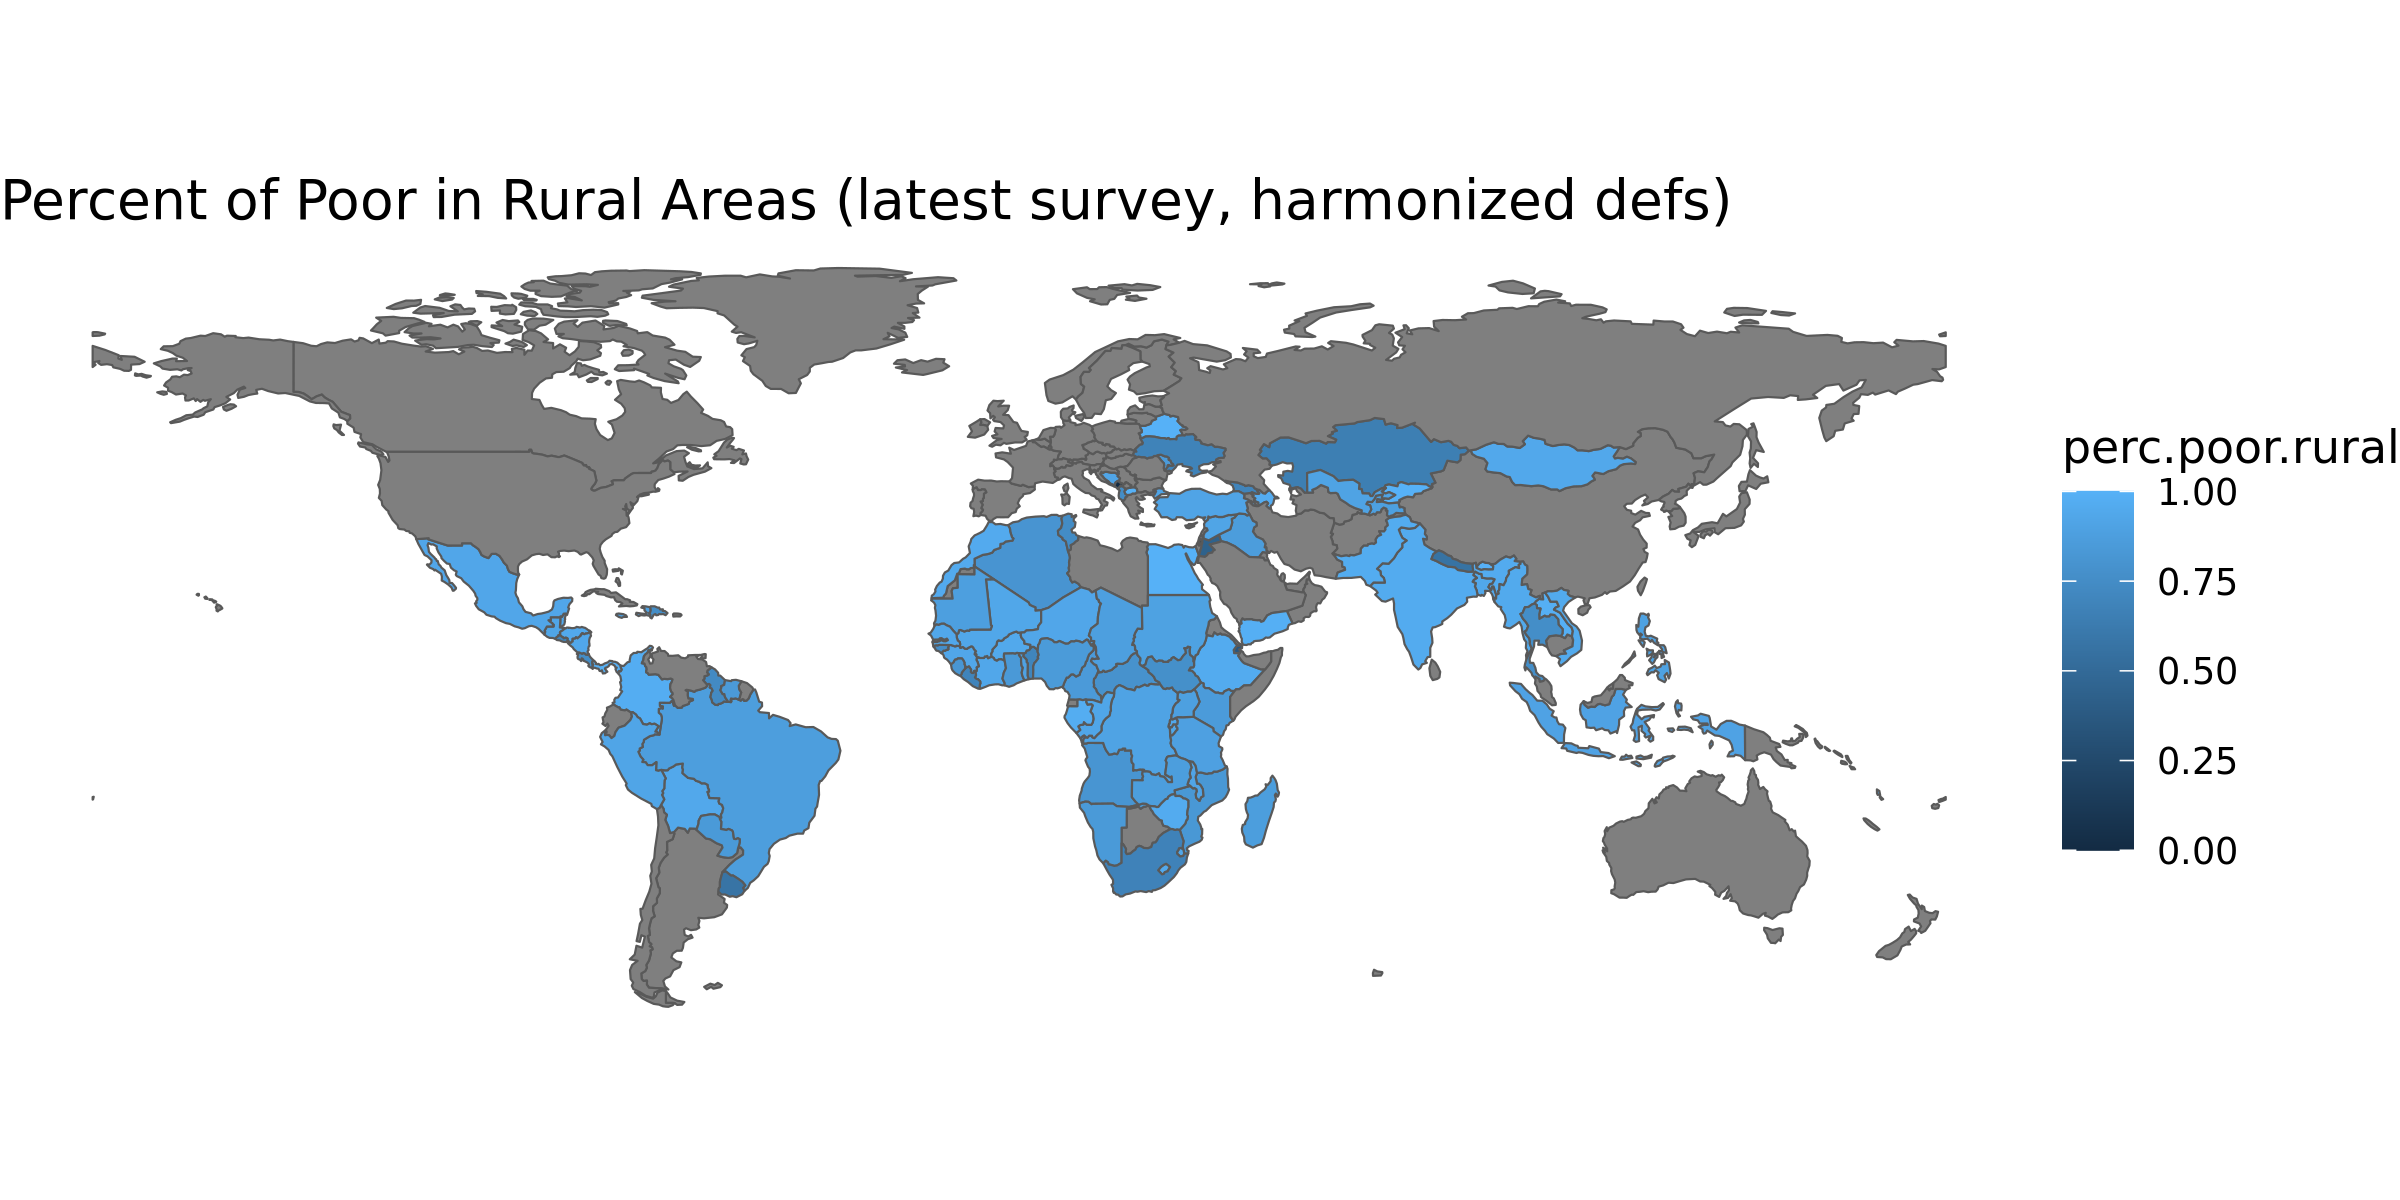
\includegraphics[width=\textwidth]{../res/perc.poor.rural_int.png}
\end{frame}

\begin{frame}
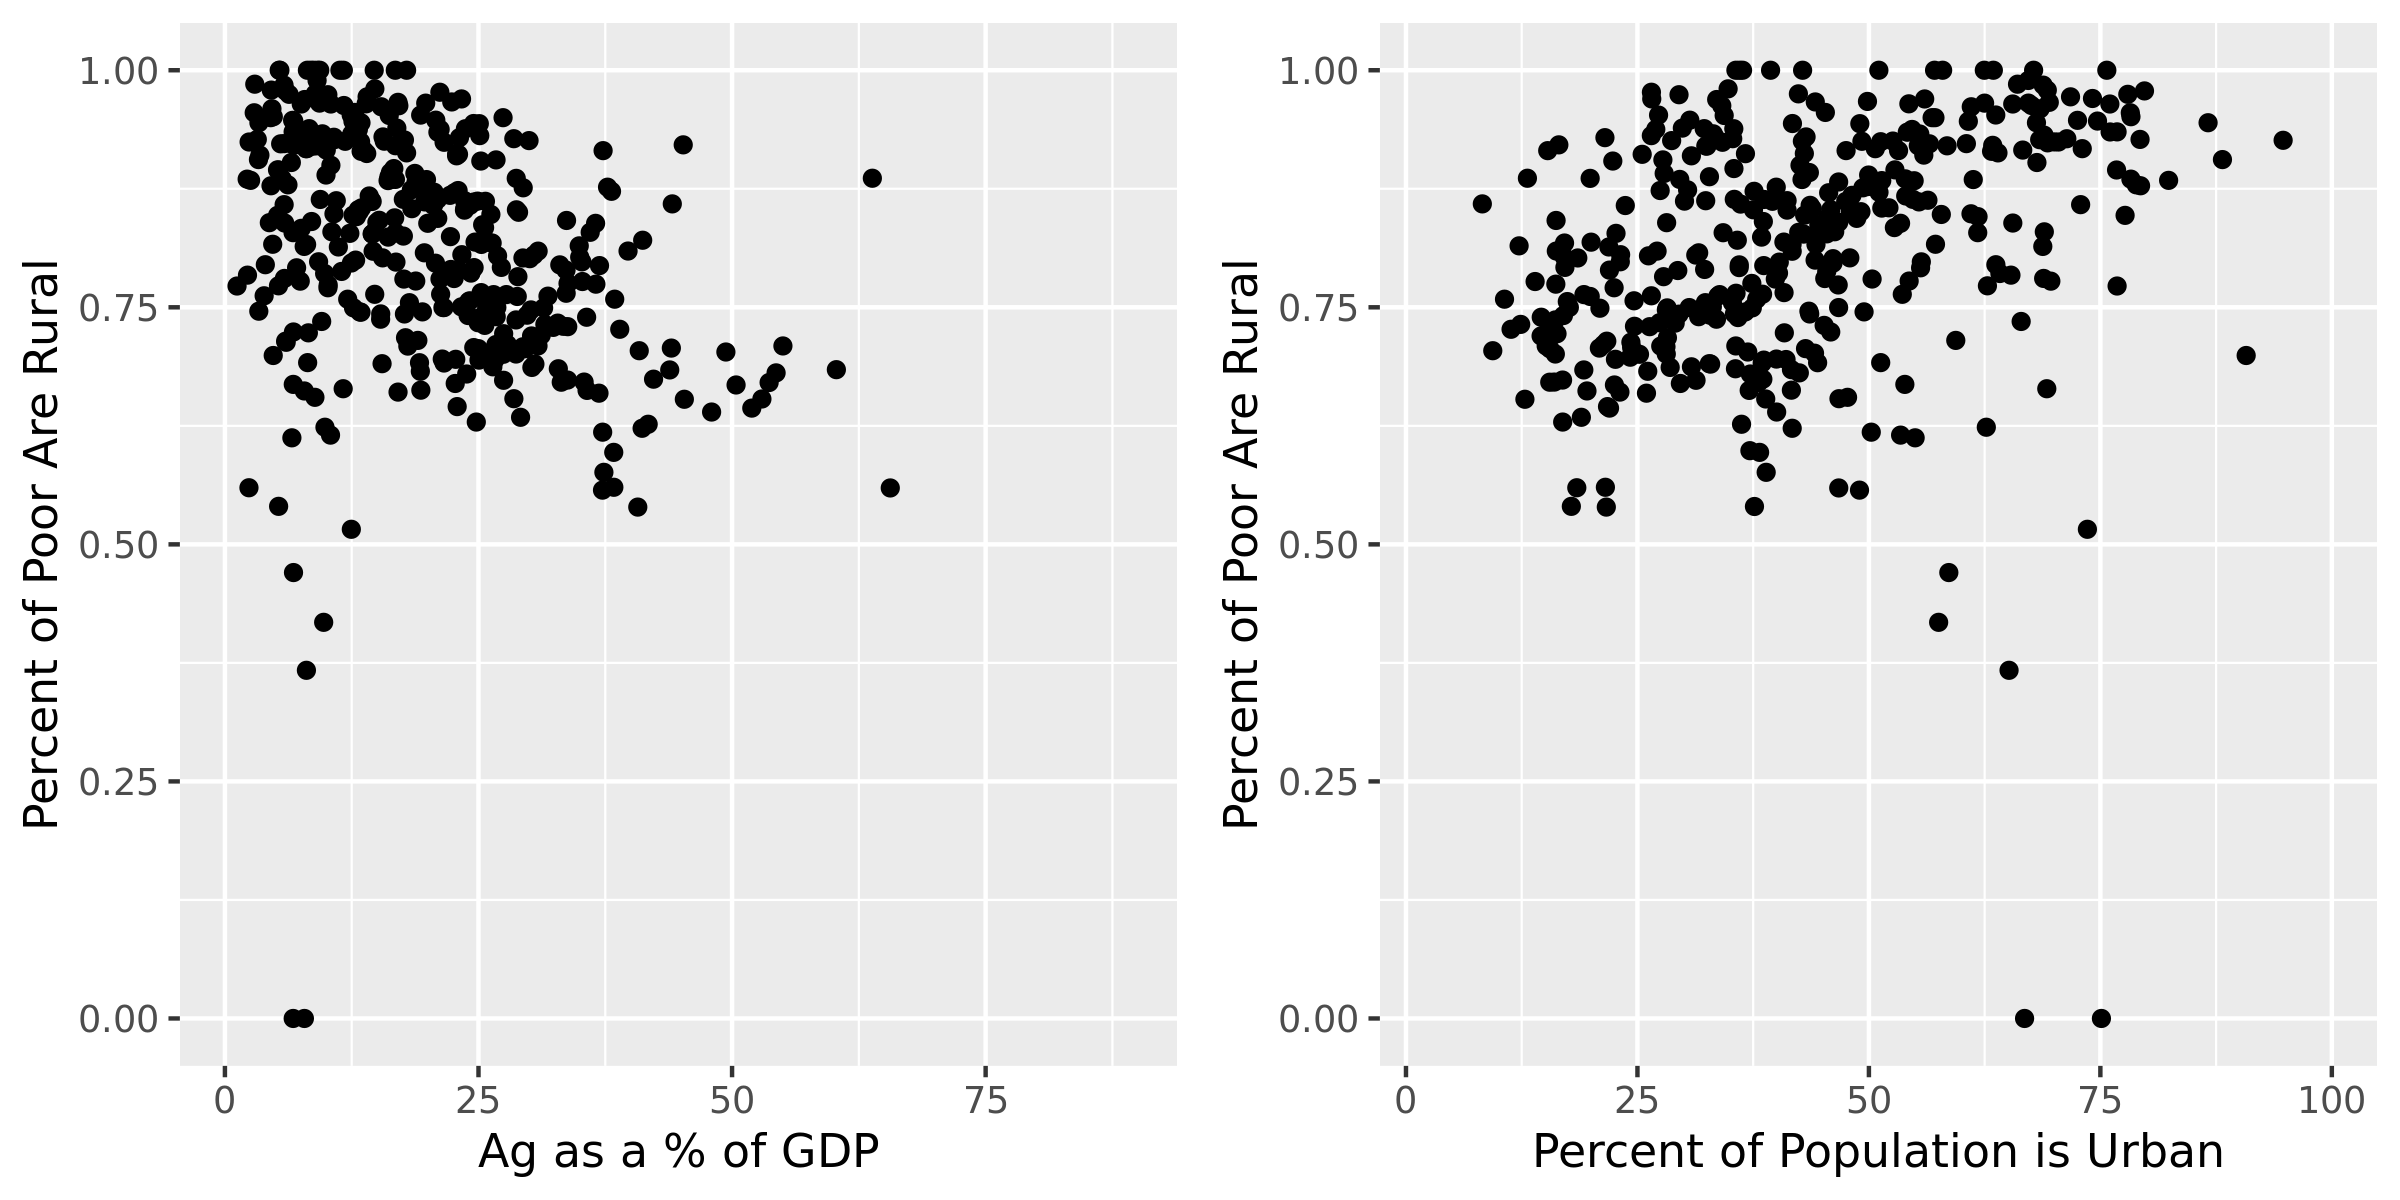
\includegraphics[width=\textwidth]{../res/Compare_other_vars.png}
\end{frame}

\end{document}
